\documentclass{article}
\usepackage[utf8]{inputenc}
\usepackage{graphicx}
\usepackage{geometry}
\geometry{a4paper, margin=1in}

\title{Osztott Rendszerek Projekt \\ Kahoot Clone}
\author{Balázs-Gudor Rózsa \\
Budai-Barabási Csanád \\
Craciun Edvin \\
Dávid Lóránd \\
Fehér Balázs Botond \\
Ivácson Attila Lénárd \\
Kántor Csongor Szilárd \\
Konya Zsófia \\
Mihácsa Gergely-Olivér \\
Szabó István \\
Szántó Róbert \\
Szántó Sándor-Norbert}
\date{\today}

\begin{document}

\maketitle

\tableofcontents

\newpage

\section{Introduction}
This document provides a detailed overview of the Kahoot Clone project, a real-time quiz game platform built with a distributed systems approach. The project is designed to handle multiple concurrent users and ensure high availability through a microservices architecture and load balancing.

\section{System Architecture}
The system is designed using a microservices architecture, which breaks down the application into smaller, independent services. This approach offers several advantages, including improved scalability, fault tolerance, and ease of maintenance.

\subsection{Architecture Diagram}
\begin{figure}[h!]
    \centering
    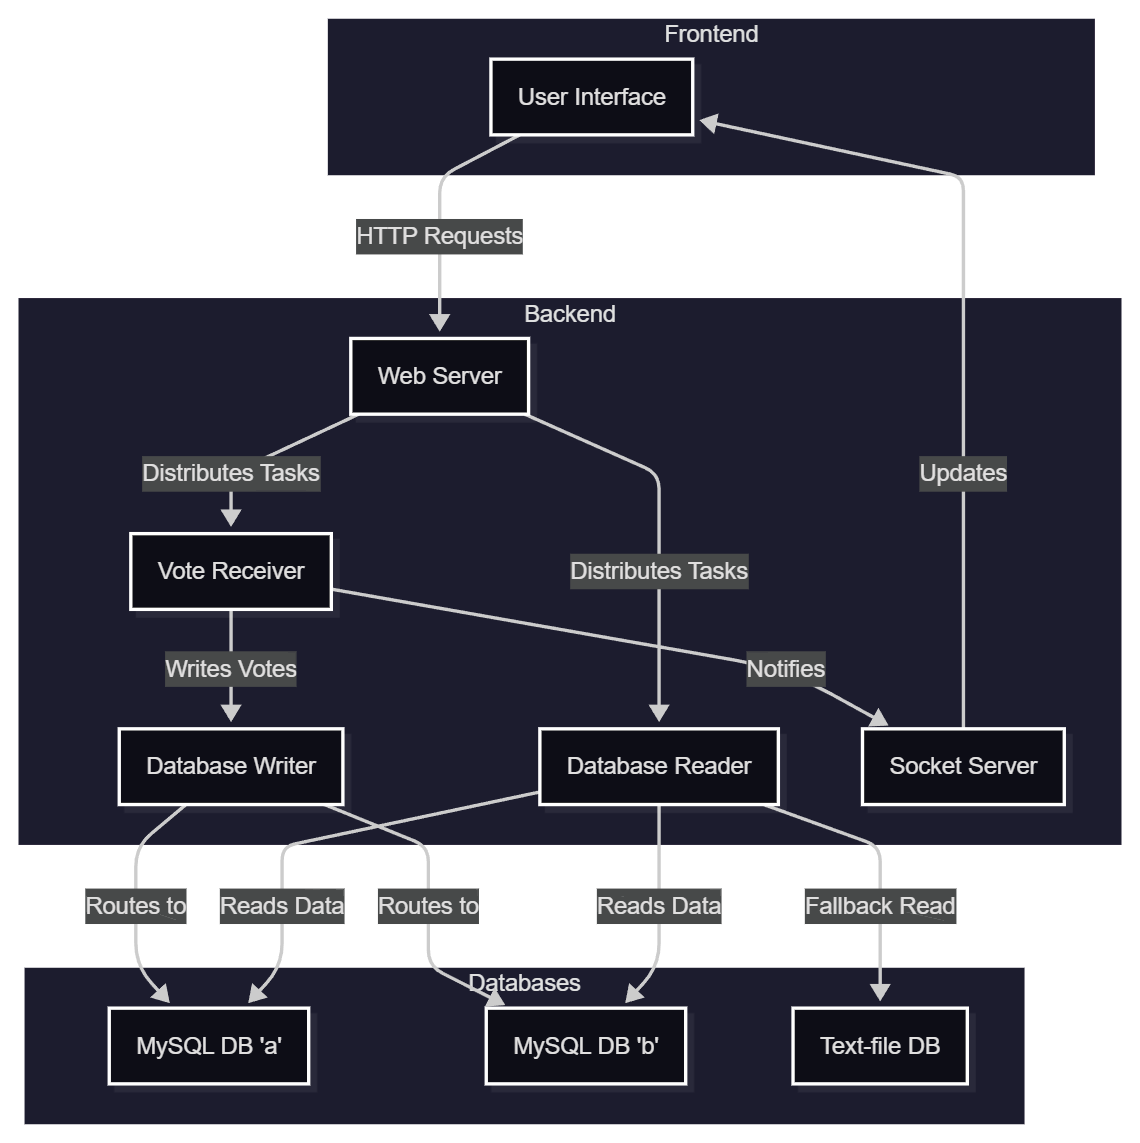
\includegraphics[width=\textwidth]{diagrams/voting_architecture.png}
    \caption{System Architecture}
\end{figure}

\subsection{Design Choices}
\subsubsection{Microservices Architecture}
We chose a microservices architecture to decouple the different functionalities of the application. This allows us to develop, deploy, and scale each service independently. For example, the Vote Receiver service can be scaled separately from the Database Reader service to handle high loads during peak times.

\subsubsection{Load Balancing}
The system uses a simple but effective load balancing strategy based on the game PIN. Even PINs are routed to one database instance, and odd PINs to another. This distributes the load evenly across the two databases.

\section{Component Breakdown}
This section provides a detailed description of each file in the project, explaining its purpose and functionality.

\subsection{Backend}
\begin{itemize}
    \item \textbf{task1\_web\_server.py}: The main entry point of the backend application.
    \item \textbf{task2\_vote\_receiver.py}: Handles incoming votes from the users.
    \item \textbf{task3\_db\_write.py}: Writes the votes to the appropriate database instance.
    \item \textbf{task4\_db\_router.py}: Routes database connections to the correct instance.
    \item \textbf{task5\_db\_read.py}: Reads data from the databases.
    \item \textbf{task6\_notify\_display.py}: Notifies the frontend when a new vote is cast.
    \item \textbf{task7\_socket\_server.py}: A TCP socket server that manages the connection with the host's display.
    \item \textbf{task8\_http\_parser.py}: Parses HTTP requests received by the socket server.
    \item \textbf{task10\_txt\_db.py}: A fallback database that uses a simple text file for storage.
    \item \textbf{task12\_results.js}: A client-side script that handles the display of results.
    \item \textbf{task14\_login.js}: Manages the user login process.
    \item \textbf{task15\_auto\_update.py}: A script that automatically updates the host's display.
\end{itemize}

\subsection{Frontend}
\begin{itemize}
    \item \textbf{index.html}: The main HTML file that structures the user interface.
    \item \textbf{task11\_gameUi.js}: This script is responsible for dynamically building the game's user interface.
    \item \textbf{task13\_styles.css}: Contains all the CSS styles for the application.
\end{itemize}

\subsection{Database}
\begin{itemize}
    \item \textbf{db\_init.sh}: A shell script that initializes the two MySQL database instances.
    \item \textbf{seed.sql}: Contains the initial data for the databases.
\end{itemize}

\section{Diagrams}

\subsection{Kahoot Clone}
This diagram provides a high-level overview of the entire Kahoot Clone application.
\begin{figure}[h!]
    \centering
    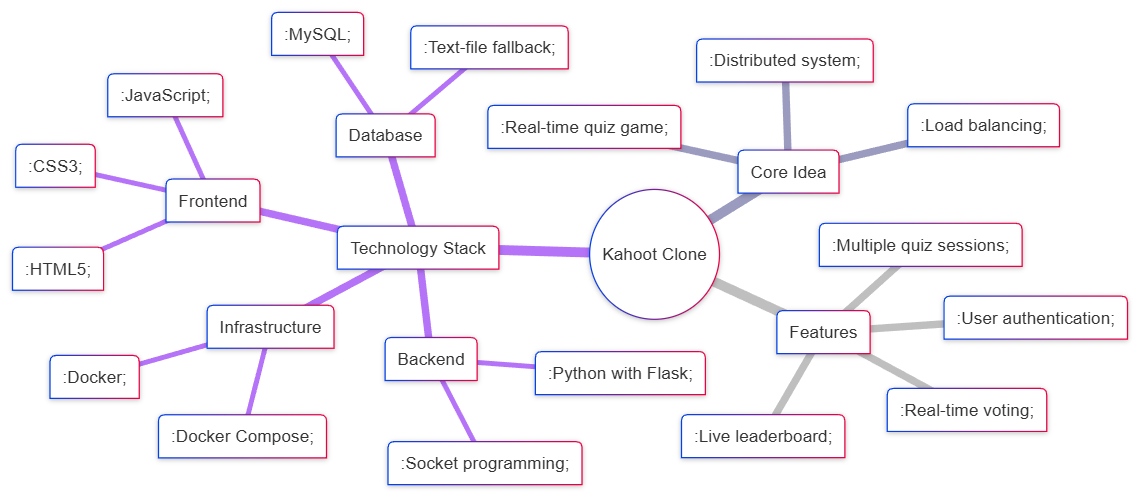
\includegraphics[width=\textwidth]{diagrams/kahoot_clone.png}
    \caption{Kahoot Clone}
\end{figure}
\clearpage

\subsection{Sequence Diagram: Vote Submission}
The following sequence diagram illustrates the process of submitting a vote, from the user's action to the database write operation. The user sends a POST request to the web server, which then delegates the vote processing to the VoteReceiver. The VoteReceiver, in turn, uses the DBWriter to persist the vote in the database.
\begin{figure}[h!]
    \centering
    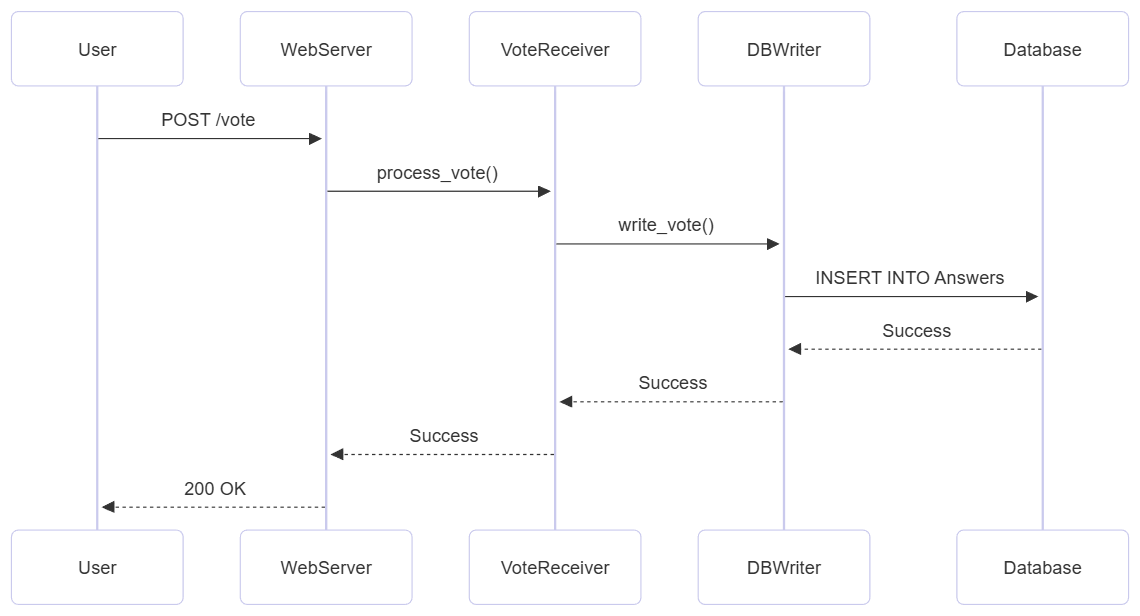
\includegraphics[width=\textwidth]{diagrams/vote_processing.png}
    \caption{Vote Submission Sequence}
\end{figure}
\clearpage

\subsection{UML Diagram}
This UML diagram describes the static structure of the system, showing the classes and their relationships.
\begin{figure}[h!]
    \centering
    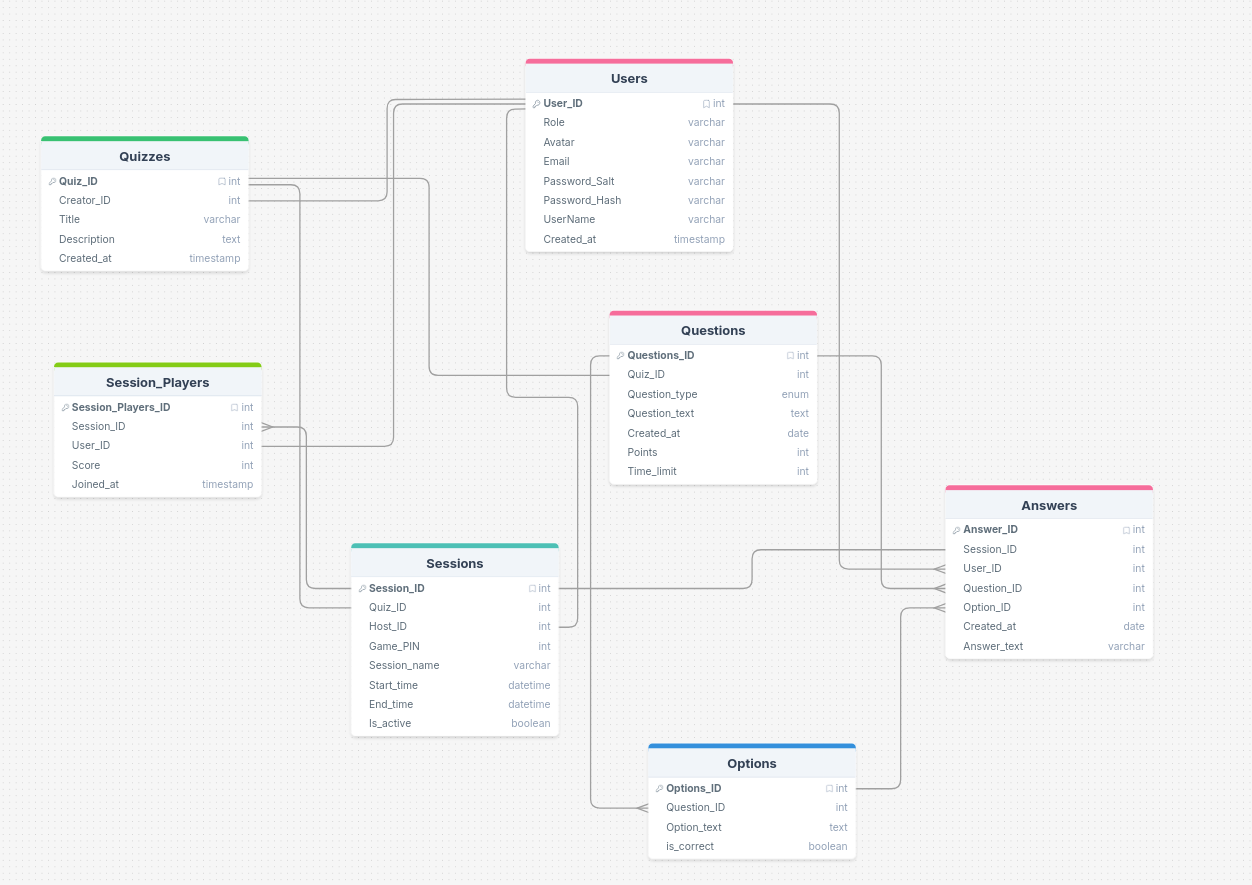
\includegraphics[width=\textwidth]{diagrams/UML_diagram.png}
    \caption{UML Diagram}
\end{figure}
\clearpage

\subsection{Game PIN Routing}
The system uses a simple but effective load balancing strategy based on the game PIN. Even PINs are routed to one database instance, and odd PINs to another. This distributes the load evenly across the two databases.
\begin{figure}[h!]
    \centering
    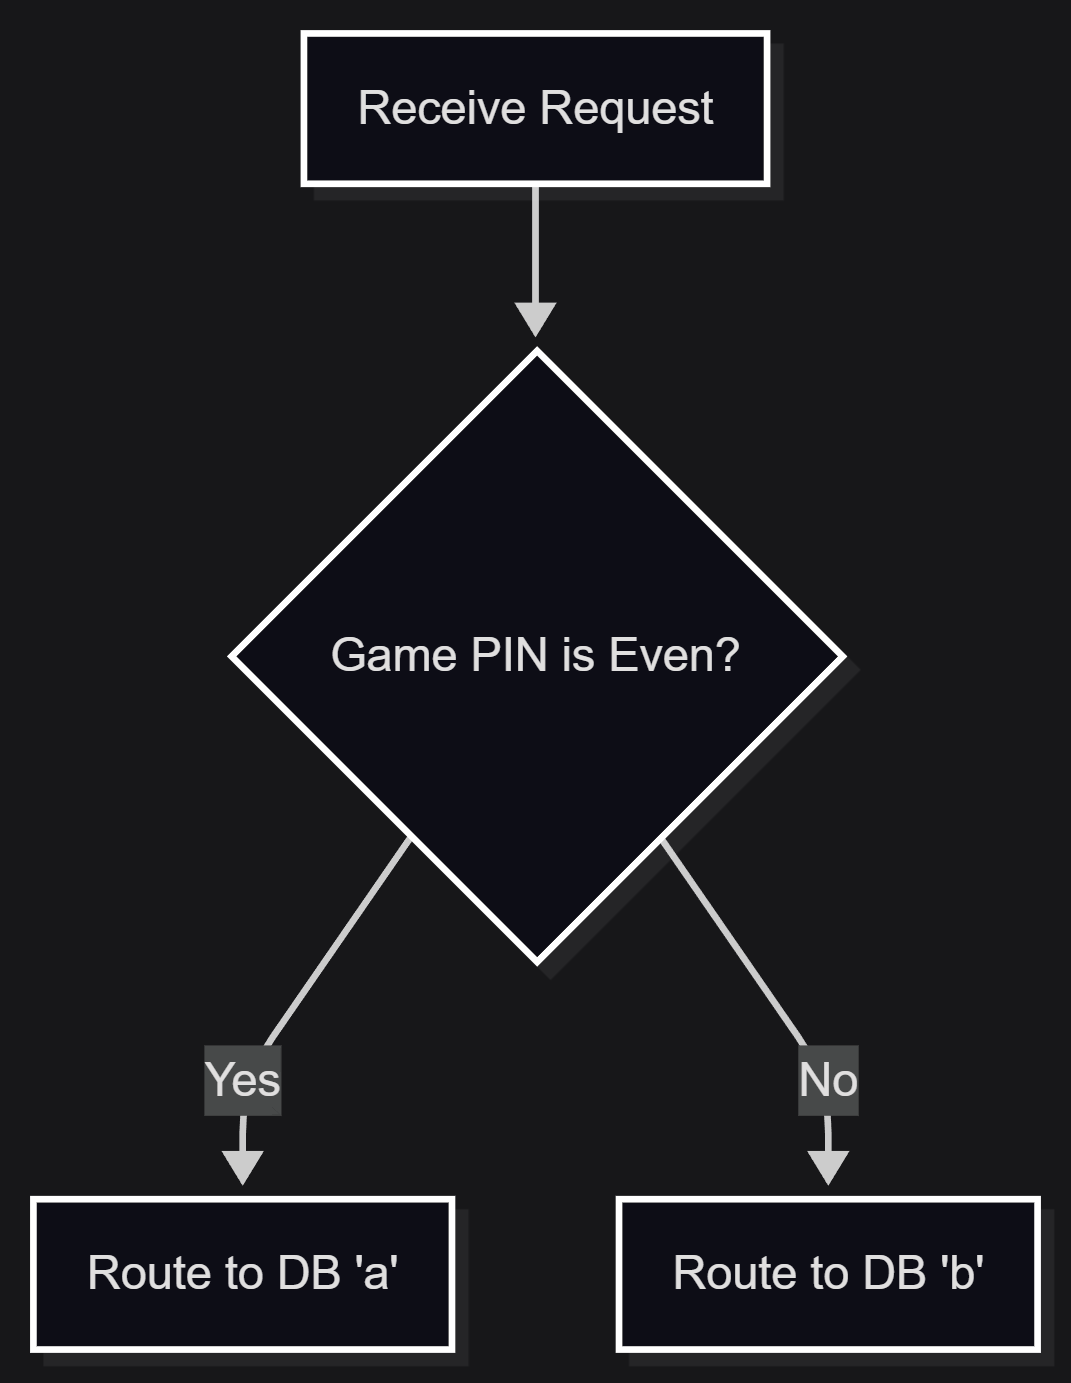
\includegraphics[width=\textwidth]{diagrams/game_pin_routing.png}
    \caption{Game PIN Routing}
\end{figure}
\clearpage

\subsection{Quiz Game}
This diagram shows the overall flow of the quiz game from the user's perspective.
\begin{figure}[h!]
    \centering
    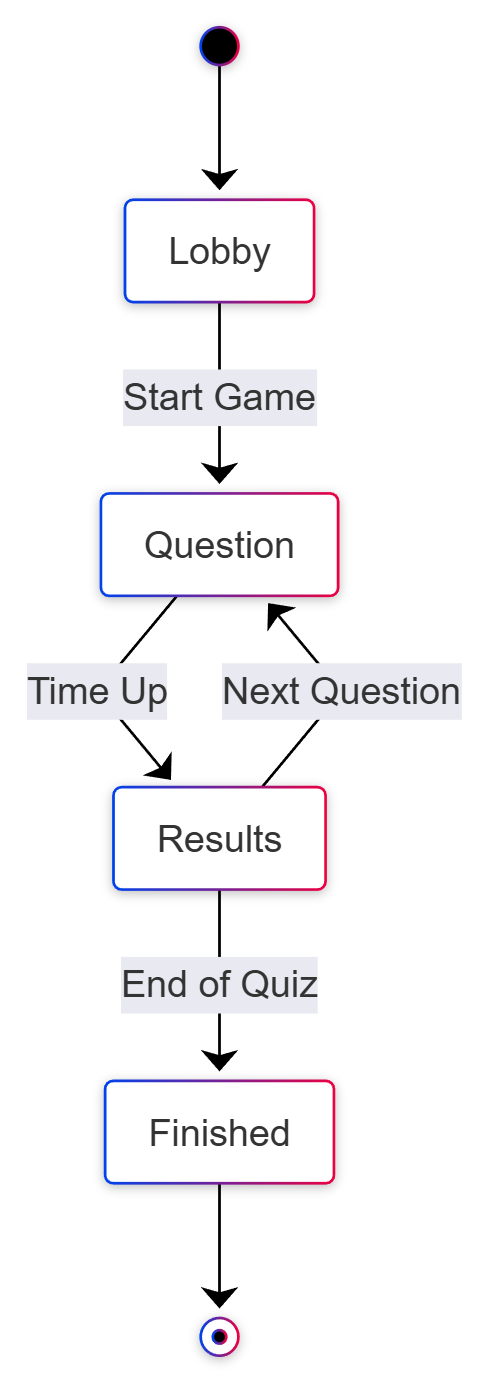
\includegraphics[width=\textwidth]{diagrams/quiz_game.png}
    \caption{Quiz Game}
\end{figure}

\end{document}
